\documentclass[UTF8,a4paper,12pt,oneside]{article}
\usepackage{ctex,amsmath,amsfonts,pgfplots,pgfplotstable}
\usepackage{geometry,graphicx,multirow,setspace}
\usepackage{caption,subcaption}
\usepackage{authblk}
\usepackage{url}
\usepackage{hyperref}
\hypersetup{hidelinks,
	colorlinks=true,
	allcolors=black,
	pdfstartview=Fit,
	breaklinks=true}
%----------------------------------------------------------------------------------------
%	COLORS
%----------------------------------------------------------------------------------------

\definecolor{color1}{RGB}{0,0,90} % Color of the article title and sections
\definecolor{color2}{RGB}{0,20,20} % Color of the boxes behind the abstract and headings

%----------------------------------------------------------------------------------------
%	HYPERLINKS
%----------------------------------------------------------------------------------------

\usepackage{hyperref} % Required for hyperlinks
\hypersetup{hidelinks,colorlinks,breaklinks=true,urlcolor=color2,citecolor=color1,linkcolor=color1,pdftitle={论文},pdfauthor={PKU 曹希哲}}
\geometry{left=2.54cm,right=2.54cm,top=3.18cm,bottom=3.18cm}
\title{计算机图形学大作业——SSAO的实现}
\author{蒋凌宇,何文阳,曹希哲}
\date{\today}
\pgfplotsset{compat=1.18}


\begin{document}
\maketitle
\section{引言}
在之前的光照模型中,我们计算了3种光照并结合到一起,分别是环境光(ambient),漫反射(diffuse),镜面反射(specular),其中对于环境光的处理较为简单,
仅仅是取为定值,即
$$ambient = ambientStrength * lightColor$$
这会带来一个问题,就是当物体形状较为复杂,表面有许多坑洼、缝隙时,这些地方应该吸收掉一部分光强,使得这一部分看上去相对较暗,而不是现在所实现的所有地方光照强度相同。
基于这样的考虑,诞生了屏幕空间环境光遮蔽技术(SSAO,Screen-Space Ambient Occlusion)。

\section{理论}
SSAO的基本原理在于对每个像素点按照半径 radius ,在其法向半球体里随机采样,计算出这些点的深度值,通过周围点的深度比例来决定该点的光照强度。
在采样的时候引入随机性,可以大大减少所需样本数量而不影响结果,因此还需要创建随机旋转纹理(noiseTexture)并平铺在屏幕上。
同时,我们对得到的结果引入偏移量,可以实现光滑的模糊遮蔽效果。最后,我们将得到的遮蔽因子引入到光照方程中,实现SSAO效果。

SSDO(Screen-Space Directional Occlusion)的原理则是在SSAO的基础上,

\section{实验}
\subsection{分工}
蒋凌宇:

何文阳:

曹希哲:负责总结实验成果,完成报告、ppt的制作

\subsection{代码细节}
首先,我们组在网上找了一个汽车的模型并导入。
\begin{figure}[!h]
    \centering
    \caption[short]{原始模型}
    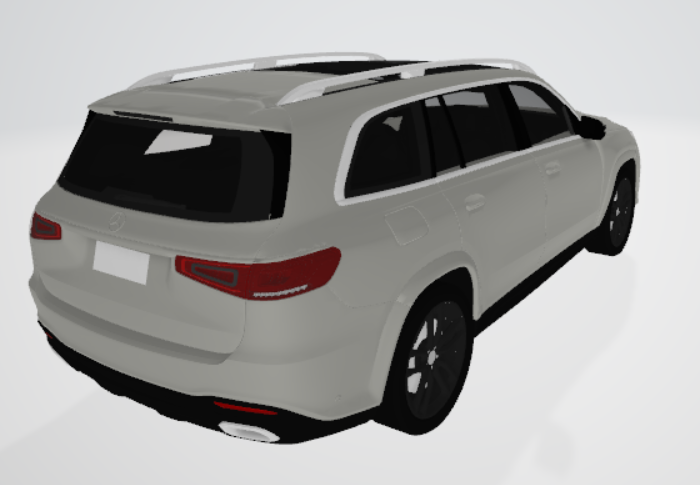
\includegraphics[scale=0.8]{Figure/model.png}
\end{figure}

然后,我们使用了3个着色器,分别是几何着色器、ssao着色器以及用于模糊遮蔽效果的ssaoBlur着色器,并将相应的纹理绑定。
在随机取样的部分,我们随机生成64个向量,x/y分量在[-1,1],z分量在[0,1],再将其全部单位化,通过这些向量,我们可以在任意像素点周围半径为1的半圆里随机取样。
同时,我们还生成了随机噪声,用于模糊遮蔽处理。

在ssao-Fragment-Shader中,我们统计了之前随机采样的点的深度,并进行判断,得到遮蔽因子(Occlusion),
并应用到环境光模型中(作为ssaoInput发送到ssaoBlur-Fragent-Shader中)。

可以看到,在应用了SSAO以后,整个模型的缝隙处变得更暗了,从而更接近人眼观察的效果。
\begin{figure}[!h]
    \centering
    \caption[short]{ssao}
    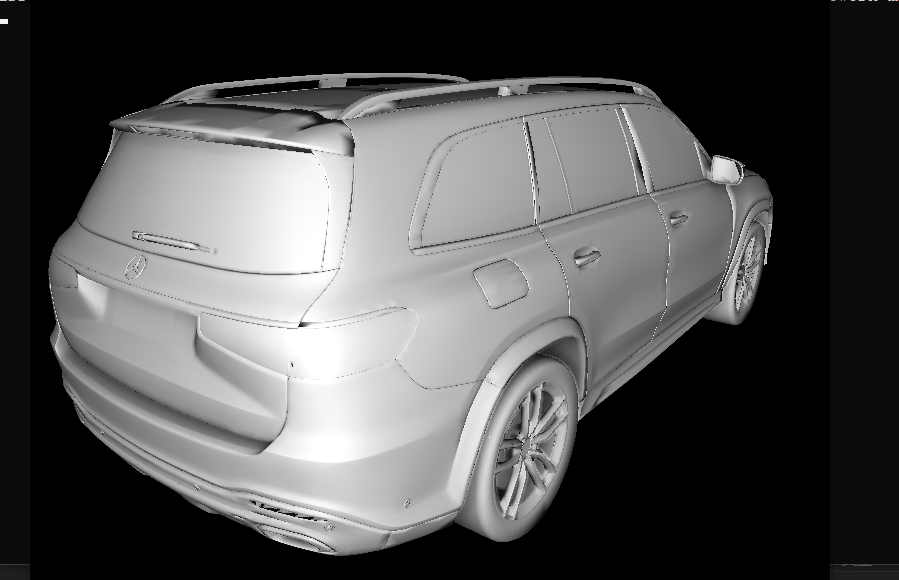
\includegraphics[scale=0.8]{Figure/ssao_result.png}
\end{figure}

\section{总结}



\section{参考文献}
链接:\href{https://learnopengl-cn.github.io/05%20Advanced%20Lighting/09%20SSAO/}{learnopengl-cn-SSAO部分}

\end{document}